\documentclass[12pt, a4paper]{article}
\usepackage{ctex}

\usepackage[margin=1in]{geometry}
\usepackage{
  color,
  clrscode,
  amssymb,
  ntheorem,
  amsmath,
  listings,
  fontspec,
  xcolor,
  supertabular,
  multirow,
  mathtools,
  mathrsfs
}
\definecolor{bgGray}{RGB}{36, 36, 36}
\usepackage[
  colorlinks,
  linkcolor=bgGray,
  anchorcolor=blue,
  citecolor=green
]{hyperref}
\newfontfamily\courier{Courier}

\theoremstyle{margin}
\theorembodyfont{\normalfont}
\newtheorem{thm}{定理}
\newtheorem{cor}[thm]{推论}
\newtheorem{pos}[thm]{命题}
\newtheorem{lemma}[thm]{引理}
\newtheorem{defi}[thm]{定义}
\newtheorem{std}[thm]{标准}
\newtheorem{imp}[thm]{实现}
\newtheorem{alg}[thm]{算法}
\newtheorem{exa}[thm]{例}
\newtheorem{prob}[thm]{问题}
\DeclareMathOperator{\sft}{E}
\DeclareMathOperator{\idt}{I}
\DeclareMathOperator{\spn}{span}
\DeclareMathOperator*{\agm}{arg\,min}
\newcommand{\pr}{\prime}
\newcommand{\tr}{^\intercal}
\newcommand{\st}{\text{s.t.}}
\newcommand{\hp}{^\prime}
\newcommand{\ms}{\mathscr}
\newcommand{\mn}{\mathnormal}
\newcommand{\tbf}{\textbf}
\newcommand{\mbf}{\mathbf}
\newcommand{\fl}{\mathnormal{fl}}
\newcommand{\f}{\mathnormal{f}}
\newcommand{\g}{\mathnormal{g}}
\newcommand{\R}{\mathbf{R}}
\newcommand{\Q}{\mathbf{Q}}
\newcommand{\JD}{\textbf{D}}
\newcommand{\rd}{\mathrm{d}}
\newcommand{\str}{^*}
\newcommand{\vep}{\varepsilon}
\newcommand{\lhs}{\text{L.H.S}}
\newcommand{\rhs}{\text{R.H.S}}
\newcommand{\con}{\text{Const}}
\newcommand{\oneton}{1,\,2,\,\dots,\,n}
\newcommand{\aoneton}{a_1a_2\dots a_n}
\newcommand{\xoneton}{x_1,\,x_2,\,\dots,\,x_n}
\newcommand\thmref[1]{定理~\ref{#1}}
\newcommand\lemmaref[1]{引理~\ref{#1}}
\newcommand\defref[1]{定义~\ref{#1}}
\newcommand\posref[1]{命题~\ref{#1}}
\newcommand\secref[1]{节~\ref{#1}}
\newcommand\equref[1]{(\ref{#1})}
\newcommand\figref[1]{图 \ref{#1}}
\newcommand\corref[1]{推论~\ref{#1}}
\newcommand\exaref[1]{例~\ref{#1}}
\newcommand\algref[1]{算法~\ref{#1}}
\newcommand{\remark}{\paragraph{评注}}
\newcommand{\example}{\paragraph{例}}
\newcommand{\proof}{\paragraph{证明}}


\title{E04a 编程作业解答}
\author{姓名:任云玮$\quad$学号:516030910586}
\date{}

\usepackage{titlesec}

\titleformat*{\section}{\large\bfseries}
\titleformat*{\subsection}{\normalsize\bfseries}
\newcommand{\ic}{\texttt}

\begin{document}
\lstset{
  numbers=left,
  basicstyle=\scriptsize,
  numberstyle=\tiny\color{red!89!green!36!blue!36},
  language=Matlab,
  breaklines=true,
  keywordstyle=\color{blue!70},commentstyle=\color{red!50!green!50!blue!50},
  morekeywords={},
  stringstyle=\color{purple},
  frame=shadowbox,
  rulesepcolor=\color{red!20!green!20!blue!20}
}
\maketitle

\paragraph{问题}由实验给出数据表.
  \begin{table}[htbp]
  \centering
  \label{数据表}
  \begin{tabular}{l|lllllll}
    \hline
    $x$ & 0.0 & 0.1  & 0.2  & 0.3  & 0.5  & 0.8  & 1.0  \\ \hline
    $y$ & 1.0 & 0.41 & 0.50 & 0.61 & 0.91 & 2.02 & 2.46 \\ \hline
  \end{tabular}
  \caption{数据表}
  \end{table}
  试求3次、4次多项式的曲线拟合,再根据数据曲线形状,求一个另外函数的拟合曲线,用图示数据曲线及相应的三种拟合曲线.

\section{多项式拟合}
\subsection{简述多项式拟合的过程}
  函数\ic{orthPoly}用于计算对于给定的样本点\ic{px}的前$n$个正交多项式,
  返回一个元胞数组,其中保存了计算得的多项式. 计算是利用递推公式
  \[
    P_{k+1}(x) = \left( x-\frac{(xP_k, P_k)}{(P_k,P_k)} \right)P_k
    - \frac{(P_k, P_k)}{(P_{k-1}, P_{k-1})}P_{k-1}.
  \]
  \par 函数\ic{orthCoefficient}用于计算对于给定的样本点\ic{(px, py)},
  和给定的正交多项式\ic{P},计算前$n$个系数. 计算是利用公式
  \[
    a_k = \frac{\sum_{i=0}^m y_iP_k(x_i)}{\sum_{i=0}^m P_k^2(x_i)}.
  \]
  \par 函数\ic{calcPoly}用于对于给定的正交多项式\ic{P}和对应的系数
  \ic{cof},计算拟合的多项式在\ic{qx}处的值. 而函数\ic{polyfitn}通过
  调用其他三个函数,计算出样本点\ic{(px, py)}对应的$n$次拟合多项式.

\subsection{编写多项式拟合的函数文件,命名为polyfitn.m}
  \lstinputlisting{../src/polyfitn.m}

\subsection{编写主程序,命名为run\_polyfitn.m,给出3次和4次的拟合,并用不同线型在同一幅图中画出拟合结果}
  见图\ref{fig: 多项式拟合}. 红色实线为三次多项式拟合,蓝色虚线为四次多项式拟合的结果。
  \begin{figure}[htbp]
    \centering
    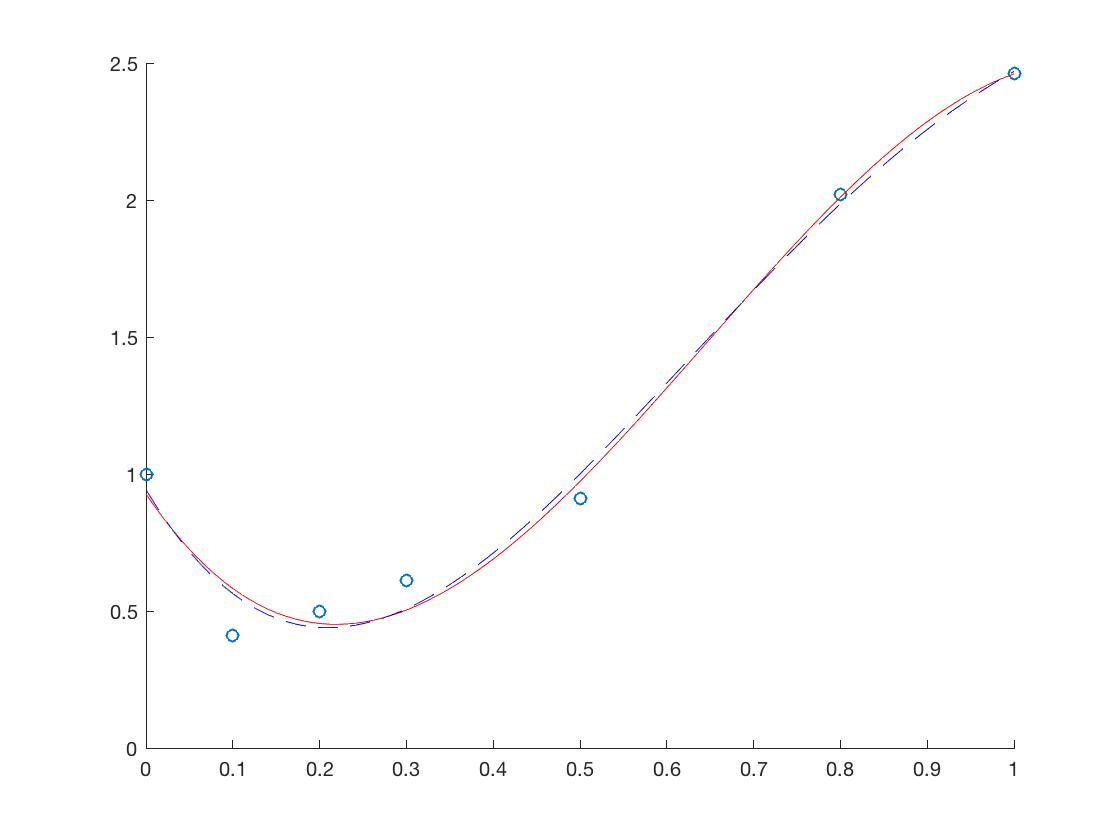
\includegraphics[height=9.9cm]{../image/run_polyfitn.jpg}
    \caption{多项式拟合结果}
    \label{fig: 多项式拟合}
  \end{figure}
  \lstinputlisting{../src/run_polyfitn.m}

\subsection{用matlab自带命令重复1.3的过程}
  见图\ref{fig: matlab多项式拟合}. 红色实线为三次多项式拟合,蓝色虚线为四次多项式拟合的结果。
  \begin{figure}
    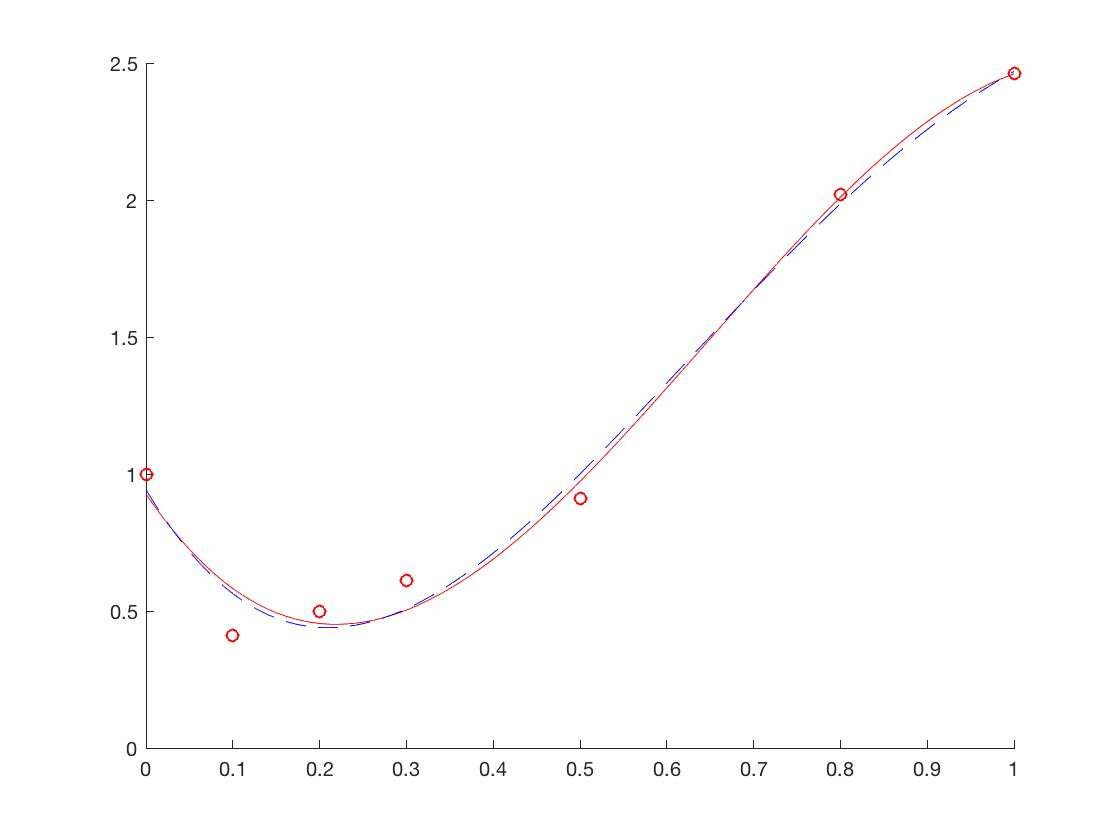
\includegraphics[height=9.9cm]{../image/run_polyfit.jpg}
    \caption{matlab多项式拟合结果}
    \label{fig: matlab多项式拟合}
  \end{figure}
  \lstinputlisting{../src/run_polyfit.m}

\section{其他函数拟合}

\subsection{图示数据曲线,猜测可能曲线,并给出拟合的求解过程}
  根据数据点,一个形如
  \[
    \f(x) = e^{P_3(x)} \,\Rightarrow\,
    \log\f(x) = P_3(x).
  \]
  的函数。对于数据点的$y$,都取$\log$,然后进行$3$次多项式拟合.

\subsection{直接编程,画出拟合图形(程序命名为run\_ployfit\_nd.m)}
见图\ref{fig: 拟合}. 红线为拟合结果.
\begin{figure}
  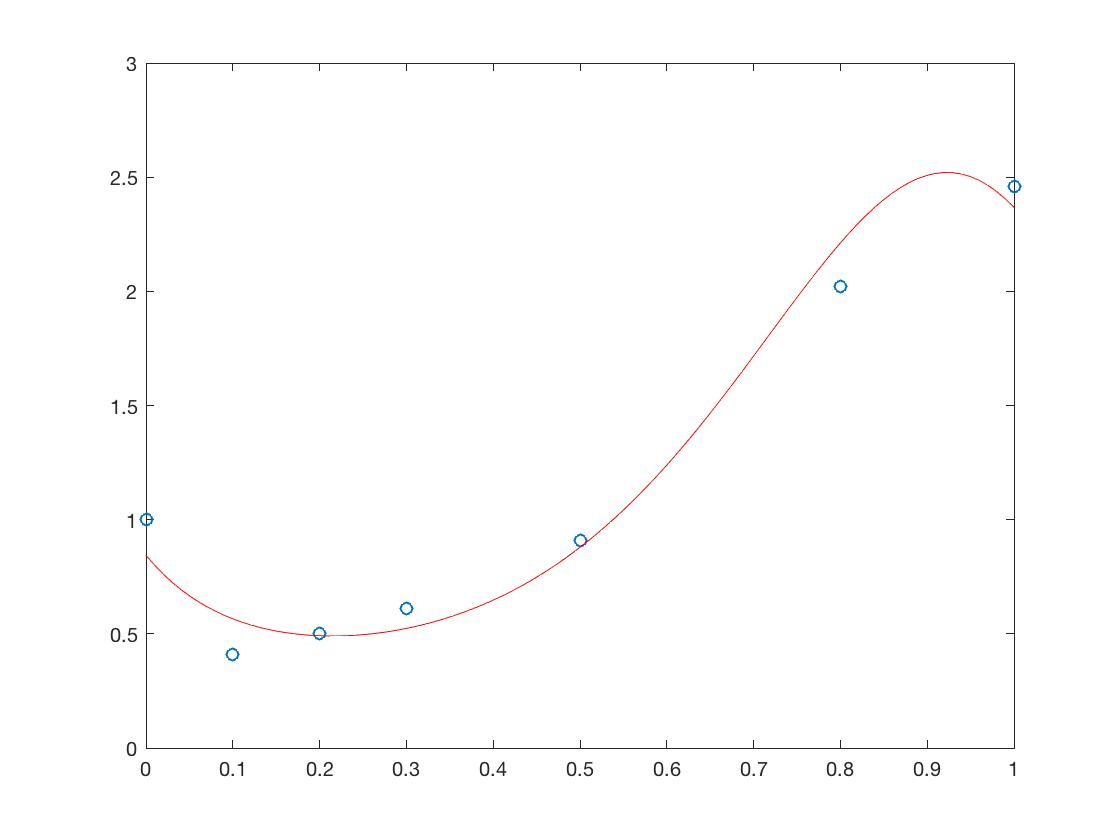
\includegraphics[height=9.9cm]{../image/run_polyfit_nd.jpg}
  \caption{拟合结果}
  \label{fig: 拟合}
\end{figure}
\lstinputlisting{../src/run_polyfit_nd.m}






\end{document}
